\newcommand{\Lagr}{\mathcal{L}}
\chapter{Modelowanie i identyfikacja}
\label{cha:model}

Wstępne obliczenia matematyczne oraz symulacje są ważnym elementem procesu projektowego umożliwiającym wczesną weryfikację przyjętych założeń. Model matematyczny oparty o wstępnie oszacowany parametry umożliwia przetestowanie projektu przed zużyciem czasu i środków na potencjalnie błędne rozwiązanie. 

\section{Model nieliniowy}
\label{nieliniowy}

Model matematyczny robota bazuje na nieliniowych równaniach różniczkowych uzyskanych przy pomocy równań Lagranga. Wyprowadzenie zostało w pełni oparte o [X] oraz zweryfikowane przy pomocy symulacji opisanej w punkcie X.X. 

\subsection{Opis matematyczny obiektu}

Przyjęte założenia: oba koła poruszają się z tą samą prędkością obrotową bez poźligu między powierzchnią koła a podłożem.

Zmienne opisujące system:


	\begin{tabular}{  l l  p{3cm} |}
		$x$& - pozioma odległość środka koła od przyjętego układu współrzędnych\\ 
		$x_c$& - pozioma odległość środka masy od przyjętego układu współrzędnych\\ 
		$z_c$& - pionowa odległość środka masy od przyjętego układu współrzędnych\\ 
		$\phi$& - położenie kątowe koła\\ 
		$\theta$& - położenie kątowe robota względem pozycji pionowej\\ 			
	\end{tabular}  



Pozostałe parametry to:


	\begin{tabular}{  l l  p{3cm} |}
		$m$& - Masa korpusu robota\\ 
		$m_w$& - Masa kół\\ 
		$R$& - Promień koła\\ 
		$L$& - Odległość pomiędzy środkiem masy a osią koła\\ 
		$\tau_0$& - zastosowany moment obrotowy\\ 
		$I$& - moment bezwładność korpusu robota\\ 
		$I_w$& - moment bezwładność kół 		\\ 	
	\end{tabular}  



Wizualizacja przyjętych symboli została przedstawiona na rysunku \ref{fig:img4_01}

\begin{figure}[h]
	\centering
	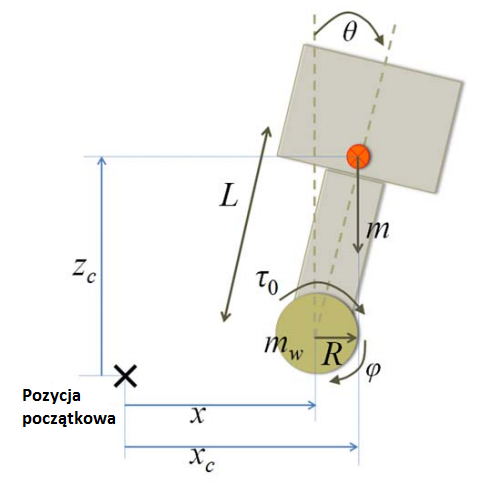
\includegraphics[scale=0.6]{img4_01.png}
	\caption{Przyjęty opis stanu obiektu}
	\label{fig:img4_01}
\end{figure}


\subsubsection{Wyprowadzenie równań modelu}
\label{wypr_rownan}
Zmienne $x, x_c, \dot{x}, \dot{x_c}, \dot{z_c} $ można zapisać jako:

\begin{equation}   x=R \phi  
\label{4row01}      \end{equation}
\begin{equation}   x_c=R \phi +Lsin\theta        \end{equation}
\begin{equation}   z_c=R +Lcos\theta       \end{equation}
\begin{equation}    \dot{x}= R \dot{\phi}      \end{equation}
\begin{equation}     \dot{x_c}= R \dot{\phi} + L\dot{\theta}cos\theta    \end{equation}
\begin{equation}  \dot{z_c}=-L\dot{\theta}sin\theta   
\label{4row06}       \end{equation}


Na podstawie równań \ref{4row01}:\ref{4row06} możemy zapisać energię potencjalną $E_p$ i kinetycznę $E_p$ w postaci \ref{4row07}:\ref{4row10}

\begin{equation}    
\label{4row07}     
E_p=mg(R+Lcos\theta)-mg(R+L)=mgl(cos\theta-1)
 \end{equation}
 \begin{equation}  E_k=1/2 m_w\dot{x}^2+1/2 I_w \dot{\phi}^2+1/2m\dot{x}_c^2+1/2m\dot{z}_c^2 +1/2mI\dot{\theta}^2   
  \end{equation}
\begin{equation} 
\label{4row10}    
 =1/2(I_w+m_wR^2+mR^2)\dot{\phi}^2 +mRLcos\theta \dot{\phi}\dot{\theta}+1/2*(I+mL^2)\dot{\theta}^2
\end{equation}

Lagranżian  $\Lagr$ może być zapisany jako różna pomiędzy energią kinetyczną a potencjalną

\begin{equation} 
\Lagr=E_k-E_p
\end{equation}
\begin{equation} 
=1/2(I_w+m_wR^2 +mR^2)\dot{\phi}^2 +mRLcos\theta\dot{\phi}\dot{\theta}+
1/2(I+mL^2)\dot{\theta}^2 +mgL(cos\theta-1)
\end{equation}

W związku z czym równania dynamiczne dla składowych $\theta$ i $\phi$ mogą zostać wyznaczone w \ref{4row11}:\ref{4row12}

\begin{equation} 
\label{4row11}    
\dfrac{\partial \Lagr}{\partial \dot{\phi}}=(I_w+m_wR^2+mR^2)\dot{\phi}+mRL\dot{\theta}cos\theta
\end{equation}
\begin{equation} 
\dfrac{\partial \Lagr}{\partial \phi}=0
\end{equation}
\begin{equation} 
\dfrac{d}{dt}(\dfrac{\partial \Lagr}{\partial \dot{\phi}})-\dfrac{\partial \Lagr}{\partial \phi}=
(I_w +m_w R^2 +mR^2)\ddot{\theta}+mRLcos\theta\ddot{\theta}-mRLsin\theta\ddot{\theta}^2=\mu
\end{equation}




\begin{equation} 
\dfrac{\partial \Lagr}{\partial \dot{\theta}}=mRLcos\theta\dot{\phi}+(I+mL^2)\dot{\theta}
\end{equation}

\begin{equation} 
\dfrac{\partial \Lagr}{\partial \theta}=-mRLsin\theta\dot{\phi}\dot{\theta}+mgLsin\theta
\end{equation}
\begin{equation} 
\label{4row12}  
\dfrac{d}{dt}(\dfrac{\partial \Lagr}{\partial \dot{\theta}})-\dfrac{\partial \Lagr}{\partial \theta}=
(I+mL^2)\ddot{\theta}+mRLcos\theta\ddot{\phi}-mRLsin\theta=\chi
\end{equation}

Gdzie $\mu$ i $\chi$ to uogólnione siły(momenty obrotowe) dla odpowiednich składowych.
Uzyskane w ten sposób równania różniczkowe można zapisać w postaci macierzowej 


\begin{equation}
\label{4row13} 
\begin{bmatrix} {I_w+(m_w+m)R^2} & {mRLcos \theta} \\{mRLcos\theta} & {I+mL^2} \end{bmatrix}
\begin{bmatrix}	\ddot{\phi}  \\	\ddot{\theta}  \end{bmatrix} +
\begin{bmatrix}	0 &-mRLsin\theta\dot{\theta} \\	0 &0 \end{bmatrix} 
\begin{bmatrix}	\dot{\phi}  \\	\dot{\theta} \end{bmatrix} +
\begin{bmatrix}	{0}  \\	{-mgLsin\theta}  \end{bmatrix} =
\begin{bmatrix}	{\mu}  \\	{\chi} \end{bmatrix}  
\end{equation}

Kolejny krok skupia się na wyrażeniu uogólnionych momentów obrotowych za pomocą znanych parametrów. Mommeny obrotowy działający na robota możemy zapisać jako sumę momentów wytworzonych przez silniki oraz rozproszonych poprzez tarcie. 


	\begin{tabular}{  l l  p{3cm} |}
	$ \tau_0 $& - łączny moment obrotowy dostarczony przez silniki \\ 
	$ \tau_a $  & -moment rozproszony poprzez tarcie w łożyskach \\ 
	$ \tau_f $  & -moment rozproszony poprzez tarcie kół o podłoże \\ 	
	$ \beta_a $  & -współczynnik tarcia w łożyskach \\ 	
	$ \beta_f $  & -współczynnik tarcia kół o podłoże \\ 	
\end{tabular}  

Po wprowadzeniu powyższych parametrów możemy zapisać uogólnione momenty obrotowe w postaci \ref{4row14}:\ref{4row15}

\begin{equation}
\label{4row14} 
\mu=\tau_0-\tau_a-\tau_f = \tau_0 -\beta_f(\dot{\phi}-\dot{\theta})-\beta_a\dot{\phi}
\end{equation}
\begin{equation}
\label{4row15} 
\chi=-\tau_0+\tau_a=-\tau_0+\beta_f(\dot{\phi}-\dot{\theta})
\end{equation}







\section{Model liniowy}

Kontrola predykcyjna opiera się na modelu liniowym wyrażonym równaniami stanu. Wprowadzony w punkcie \ref{nieliniowy} model robota jest nieliniowy, w związku z czym, wymaga on linearyzacji w punkcie równowagi. Jako punkt linearyzacji modelu wybrany został górny, niestabliny punkt równowagi.

Do w celu umożliwienia linearyzacji koniecznie były następujące uproszczenia:
\begin{itemize}
	\item  Niewielki zakres ruchów względem pozycji pionowej 
	\item  $cos\theta \approx 1$
	\item  $sin\theta \approx 0$
\end{itemize}

Równania modelu \ref{4row14} po wprowadzeniu tej modyfikacji przedstawione zostały jako równanie \ref{4row16}.

\begin{equation}
\label{4row16} 
\begin{bmatrix} {I_w+(m_w+m)R^2} & {mRL} \\{mR} & {I+mL^2} \end{bmatrix}
\begin{bmatrix}	\ddot{\phi}  \\	\ddot{\theta}  \end{bmatrix} +
\begin{bmatrix}	\beta_a + \beta_f &-\beta_f \\	-\beta_f &\beta_f \end{bmatrix} 
\begin{bmatrix}	\dot{\phi}  \\	\dot{\theta} \end{bmatrix} +
\begin{bmatrix}	{0}  \\	{-mgL}  \end{bmatrix}\theta =
\begin{bmatrix}	{1}  \\	{-1} \end{bmatrix}  \tau_0
\end{equation}


Równanie \ref{4row16} można przedstawić w zwięzłym stylu w postaci \ref{4row18}

\begin{equation}
\label{4row18} 
E
\begin{bmatrix}	\ddot{\phi}  \\	\ddot{\theta}  \end{bmatrix} +
F
\begin{bmatrix}	\dot{\phi}  \\	\dot{\theta} \end{bmatrix} +
G\theta
=H\tau_0
\end{equation}

Na postawie równania \ref{4row18} możemy zapisać model systemu w postaci równań stanu. Jako zmienne stanu wykorzystane zostaną $\phi, \theta, \dot{\phi}, \dot{\theta}$. Wejściem systemu jest moment obrotowy $\tau_0$. Jako wyjścia zostały wybrane przemieszczenie robota w osi $x$ oraz położenie kątowe korpusu $\theta$. W związku z tymi założeniami równania stanu systemu przyjmują postać  \ref{4row19} :\ref{4row20} 

\begin{equation}
\label{4row19} 
\frac{d}{dt}
\begin{bmatrix}	\phi \\ \theta \\ \dot{\phi}  \\	\dot{\theta}  \end{bmatrix} 
=
TO_DUZE
\begin{bmatrix}		\phi \\ \theta \\\dot{\phi}  \\	\dot{\theta} \end{bmatrix} +
\begin{bmatrix}	0 \\ 0 \\ \dot{\phi}  \\	\dot{\theta} \end{bmatrix}
\tau_0
\end{equation}

\begin{equation}
\label{4row20} 
y=
\begin{bmatrix}	R & 0  & 0&0 \\ 0 & 1 & 0 & 0 \end{bmatrix} 
\begin{bmatrix}	\phi \\ \theta \\ \dot{\phi}  \\	\dot{\theta}  \end{bmatrix} 
\end{equation}


Przyjmując standardową nomenklaturę teorii sterowania finalna postać rownań stanu została przedstawiona za pomocą równań: \ref{4row21} :\ref{4row22} 

\begin{equation}
\label{4row21} 
\frac{d}{dt}
x=Ax+B\tau_0
\end{equation}

\begin{equation}
\label{4row22} 
y=Cx
\end{equation}



\section{Symulacja oraz wizualizacja wyników}

Symulacja zachowania robota w oparciu o wprowadzony w punkcie \ref{wypr_rownan} model została zaimplementowana w pakiecie Matlab Simulink. Implementacja została wykorzystana do weryfikacji poprawności modelu nieliniowego, jako test planowanych rozwiązań sprzętowych oraz regulatora. Zrzut ekranu zawierający główną częśc symulacji został przedstawiony na rysunku\ref{fig:non_lin_sim} 

\begin{figure}[h]
	\centering
	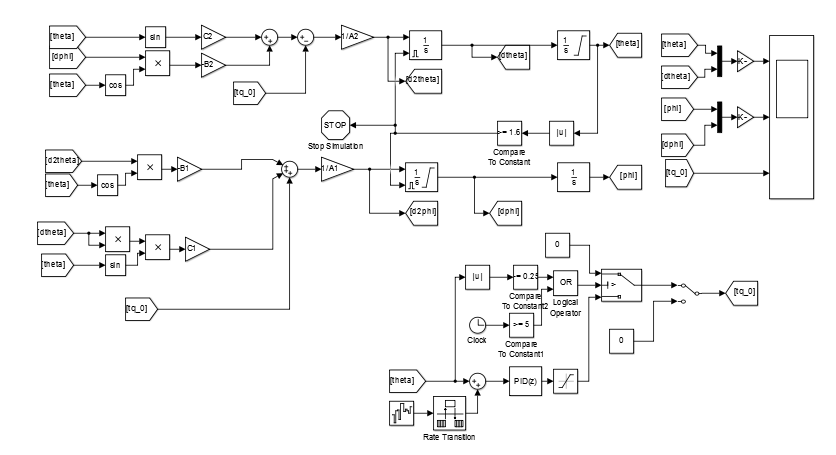
\includegraphics[scale=0.6]{sim_non_lin.PNG}
	\caption{Symulacja modelu nieliniowego}
	\label{fig:non_lin_sim}
\end{figure}

Przed każdym uruchomieniem można wybrać wartości początkowe podstawowych parametrów takich jak prędkość i pozycja kątowa koła oraz korpusu oraz nastawy regulatora i czas symulacji.
Parametry modelu ustawiane są w niezależnym skrypcie uruchamianym przed każdą symulacją. Po symulacji wykonywany jest skrypt wyrysowywujący przebiegi kluczowych zmiennych oraz prosta animacja wizualizująca przebieg symulacji.Pozwala to na szybką ocenę czy zachowanie modelu jest bliskie rzeczywistości. Przykładowy wynik symulacji został zaprezentowany na rysunku \ref{fig:non_lin_res} 

\begin{figure}[h]
	\centering
	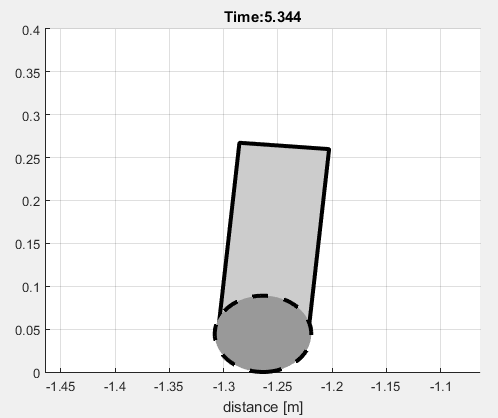
\includegraphics[scale=0.8]{visualisation_non_lin.PNG}
	\caption{Symulacja modelu nieliniowego}
	\label{fig:non_lin_res}
\end{figure}